% !TeX spellcheck = en_US
\documentclass{article}

\usepackage[english]{babel}
\usepackage[utf8]{inputenc}
\usepackage{amsmath}
\usepackage{graphicx}
\usepackage{float}
\usepackage{breqn}


\usepackage{fullpage}
\usepackage{pdfpages}
\usepackage{color}
\usepackage{amsmath}
\usepackage{url}
\usepackage{verbatim}
\usepackage{graphicx}
\usepackage{parskip}
\usepackage{amssymb}
\usepackage{nicefrac}
\usepackage{listings} % For displaying code
\usepackage{algorithm2e} % pseudo-code

\def\rubric#1{\gre{Rubric: \{#1\}}}{}

% Colors
\definecolor{blu}{rgb}{0,0,1}
\def\blu#1{{\color{blu}#1}}
\definecolor{gre}{rgb}{0,.5,0}
\def\gre#1{{\color{gre}#1}}
\definecolor{red}{rgb}{1,0,0}
\def\red#1{{\color{red}#1}}
\def\norm#1{\|#1\|}

% Math
\def\R{\mathbb{R}}
\def\argmax{\mathop{\rm arg\,max}}
\def\argmin{\mathop{\rm arg\,min}}
\newcommand{\mat}[1]{\begin{bmatrix}#1\end{bmatrix}}
\newcommand{\alignStar}[1]{\begin{align*}#1\end{align*}}
\def\half{\frac 1 2}
\def\cond{\; | \;}

% LaTeX
\newcommand{\fig}[2]{\includegraphics[width=#1\textwidth]{#2}}
\newcommand{\centerfig}[2]{\begin{center}\includegraphics[width=#1\textwidth]{#2}\end{center}}
\newcommand{\matCode}[1]{\lstinputlisting[language=Matlab]{a2f/#1.m}}
\def\items#1{\begin{itemize}#1\end{itemize}}
\def\enum#1{\begin{enumerate}#1\end{enumerate}}


\begin{document}

\title{CPSC 340/532M Assignment 1}
\author{Zhanbing Xiao/94837168; He Zhang/83857169}
\date{Sep/2018}
\maketitle
\maketitle
\vspace{-4em}

\section*{Instructions}
\rubric{mechanics:5}

The above points are allocated for compliance with the CPSC 340 homework submission instructions:\\
\url{https://github.ugrad.cs.ubc.ca/CPSC340-2018W-T1/home/blob/master/homework_instructions.md}



\section{Training and Testing}
If you run \texttt{python main.py \string-q 1}, it will load the \emph{citiesSmall.pkl} data set from Assignment 1.
Note that this file contains not only training data, but also test data, \texttt{X\string_test} and \texttt{y\string_test}.
After training a depth-2 decision tree with the information gain splitting rule, it will evaluate the performance of the classifier on the test data.
With a depth-2 decision tree, the training and test error are fairly close, so the model hasn't overfit much.

\subsection{Training and Testing Error Curves}
\rubric{reasoning:2}

\blu{Make a plot that contains the training error and testing error as you vary the depth from 1 through 15. How do each of these errors change with the decision tree depth?}

Note: it's OK to reuse code from Assignment 1.

\gre{
Answer:
\begin{itemize}
\item Refer to the following figure.
\item Both training error and test error decrease as tree depth increases. The decreasing rate is slower with tree depth increasing for both errors. However, eventually, training error decreases to 0 while testing error decreases to certain level and keeps flat.
\end{itemize}
}

\begin{figure}[H]
\centering
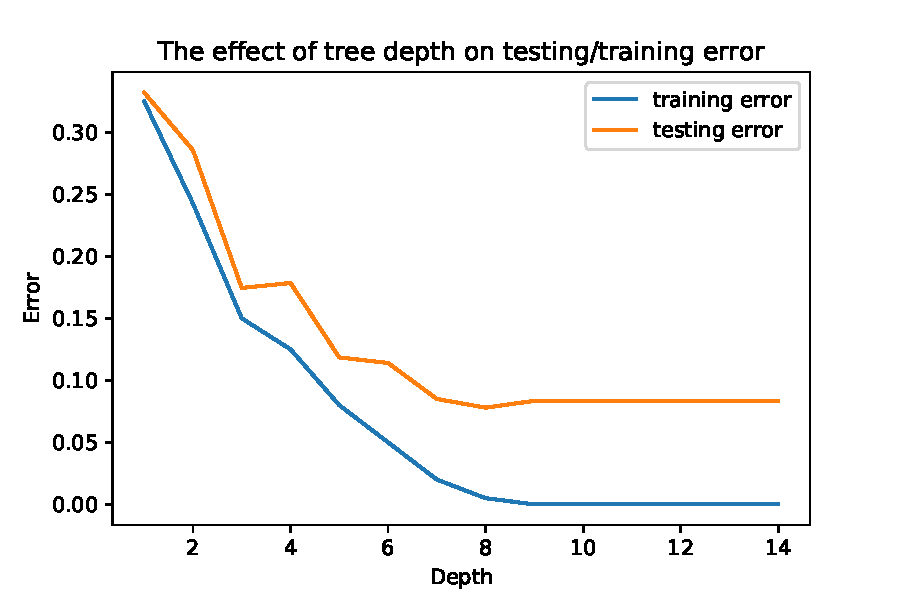
\includegraphics[width=3in]{../figs/q1_1_TrainTest}
\end{figure}


\subsection{Validation Set}
\rubric{reasoning:3}

Suppose that we didn't have an explicit test set available. In this case, we might instead use a \emph{validation} set. Split the training set into two equal-sized parts: use the first $n/2$ examples as a training set and the second $n/2$ examples as a validation set (we're assuming that the examples are already in a random order). \blu{What depth of decision tree would we pick to minimize the validation set error? Does the answer change if you switch the training and validation set? How could use more of our data to  estimate the depth more reliably?}

\gre{
Answer:
\begin{itemize}
\item The optimal depth is 8 with the first half data as training data and 6 with the second half as training data.
\item We could use cross validation to make the estimate more reliable.
\end{itemize}
}

\section{Naive Bayes}

In this section we'll implement naive Bayes, a very fast classification method that is often surprisingly accurate for text data with simple representations like bag of words.



\subsection{Naive Bayes by Hand}

Consider the dataset below, which has $10$ training examples and $3$ features:
\[
X = \begin{bmatrix}0 & 0 & 1\\0 & 1 & 1\\ 0 & 1 & 1\\ 1 & 1 & 0\\0 & 1 & 0\\0 & 1 & 1\\1 & 0 & 0\\1 & 1 & 0\\1 & 0 & 1\\1 & 0 & 0\\\end{bmatrix}, \quad y = \begin{bmatrix}\text{spam}\\\text{spam}\\\text{spam}\\\text{spam}\\\text{spam}\\\text{spam}\\\text{not spam}\\\text{not spam}\\\text{not spam}\\\text{not spam}\end{bmatrix}.
\]
The feature in the first column is $<$your name$>$ (whether the e-mail contained your name), in the second column is ``pharmaceutical'' (whether the e-mail contained this word), and the third column is ``PayPal'' (whether the e-mail contained this word).
Suppose you believe that a naive Bayes model would be appropriate for this dataset, and you want to classify the following test example:
\[
\hat{x} = \begin{bmatrix}1 & 1 & 0\end{bmatrix}.
\]

\subsubsection{Prior probabilities}
\rubric{reasoning:1}
\blu{Compute the estimates of the class prior probabilities} (you don't need to show any work):
\items{
\item$ p(\text{spam})$.\\
 \gre{ Answer: $\frac{6}{10}$ }
\item $p(\text{not spam})$. \\
 \gre{Answer: $\frac{4}{10}$}
}

\subsubsection{Conditional probabilities}
\rubric{reasoning:1}

\blu{Compute the estimates of the 6 conditional probabilities required by naive Bayes for this example}  (you don't need to show any work):
\items{
\item $p(\text{$<$your name$>$} = 1  \cond \text{spam})$. \\
\gre{Answer:$\frac{1}{6}$}
\item $p(\text{pharmaceutical} = 1 \cond \text{spam})$.\\
\gre{Answer:$\frac{5}{6}$}
\item $p(\text{PayPal} = 0  \cond \text{spam})$.\\
\gre{Answer:$\frac{1}{3}$}
\item $p(\text{$<$your name$>$} = 1  \cond \text{not spam})$.\\
\gre{Answer:$1$}
\item $p(\text{pharmaceutical} = 1  \cond \text{not spam})$.\\
\gre{Answer:$\frac{1}{4}$}
\item $p(\text{PayPal} = 0  \cond \text{not spam})$.\\
\gre{Answer:$\frac{3}{4}$}
}

\subsubsection{Prediction}
\rubric{reasoning:1}

\blu{Under the naive Bayes model and your estimates of the above probabilities, what is the most likely label for the test example? (Show your work.)}

\gre{
Answer:
\begin{eqnarray*}
p(x_1=1, x_2=1, x_3=0|spam)*p(spam) &=& p(x_1=1|spam)*p(x_2=1|spam)*p(x_3=0|spam)*p(spam) \\
&=&  (\frac{1}{6})*(\frac{5}{6})*(\frac{1}{3})*(\frac{6}{10})\\
&=& \frac{1}{36}.
\end{eqnarray*}
}
\gre{
\begin{eqnarray*}
&&p(x_1=1, x_2=1, x_3=0|not spam)*p(not spam) \\
&=& p(x_1=1|not spam)*p(x_2=1|not spam)*p(x_3=0|not spam)*p(not spam) \\
&=&  (1)*(\frac{1}{4})*(\frac{3}{4})*(\frac{4}{10}) \\
&=& \frac{3}{40} .
\end{eqnarray*}
}

\gre{Since $p(x_1=1, x_2=1, x_3=0|spam)*p(spam)<p(x_1=1, x_2=1, x_3=0|not spam)*p(not spam)$, we predict "not spam".}

\subsubsection{Laplace smoothing}
\label{laplace.conceptual}
\rubric{reasoning:2}

One way to think of Laplace smoothing is that you're augmenting the training set with extra counts. Consider the estimates of the conditional probabilities in this dataset when we use Laplace smoothing (with $\beta = 1$).
\blu{Give a set of extra training examples that we could add to the original training set that would make the basic estimates give us the estimates with Laplace smoothing} (in other words give a set of extra training examples that, if they were included in the training set and we didn't use Laplace smoothing, would give the same estimates of the conditional probabilities as using the original dataset with Laplace smoothing).
Present your answer in a reasonably easy-to-read format, for example the same format as the data set at the start of this question.

\gre{Answer:
\[
X = \begin{bmatrix}0 & 0 & 0\\1 & 1 & 1\\ 0 & 0 & 0\\ 1 & 1 & 1\\\end{bmatrix}, \quad y = \begin{bmatrix}\text{spam}\\\text{spam}\\\text{not spam}\\\text{not spam}\end{bmatrix}.
\] }


\subsection{Bag of Words}
\rubric{reasoning:3}

If you run \texttt{python main.py -q 2.2}, it will load the following dataset:
\enum{
\item $X$: A binary matrix. Each row corresponds to a newsgroup post, and each column corresponds to whether a particular word was used in the post. A value of $1$ means that the word occured in the post.
\item $wordlist$: The set of words that correspond to each column.
\item $y$: A vector with values $0$ through $3$, with the value corresponding to the newsgroup that the post came from.
\item $groupnames$: The names of the four newsgroups.
\item $Xvalidate$ and $yvalidate$: the word lists and newsgroup labels for additional newsgroup posts.
}
\blu{Answer the following}:
\enum{
\item Which word corresponds to column 51 of $X$? (This is column 50 in Python.)\\
\quad \gre{Answer: "lunar"}
\item Which words are present in training example 501? \\
\quad \gre{Answer: "car"; "fact"; "gun"; "video".}
\item Which newsgroup name does training example 501 come from? \\
\quad \gre{Answer: "talk.*".}
}

\subsection{Naive Bayes Implementation}
\rubric{code:5}

If you run \texttt{python main.py -q 2.3}
it will load the newsgroups dataset, fit a basic naive Bayes model and report the validation error.

The \texttt{predict()} function of the naive Bayes classifier is already implemented.
However, in \texttt{fit()}
the calculation of the variable \texttt{p\_xy} is incorrect
(right now, it just sets all values to $1/2$).
\blu{Modify this function so that \texttt{p\_xy} correctly
computes the conditional probabilities of these values based on the
frequencies in the data set. Submit your code and the validation error that you obtain.
Also, compare your validation error to what you obtain with scikit-learn's implementation, \texttt{BernoulliNB}.}

\gre{Answer:
\begin{itemize}
	\item Refer to "naive_bayes.py" for code details.
	\item The validation error now is 0.188. It's pretty close to the validation error from scikit-learn's BernoulliNB, which is 0.187. They are almost the same.
\end{itemize}}


\subsection{Runtime of Naive Bayes for Discrete Data}
\rubric{reasoning:3}

For a given training example $i$, the predict function in the provided code computes the quantity
\[
p(y_i \cond x_i) \propto p(y_i)\prod_{j=1}^d p(x_{ij} \cond y_i),
\]
for each class $y_i$ (and where the proportionality constant is not relevant). For many problems, a lot of the $p(x_{ij} \cond y_i)$ values may be very small. This can cause the above product to underflow. The standard fix for this is to compute the logarithm of this quantity and use that $\log(ab) = \log(a)+\log(b)$,
\[
\log p(y_i \cond x_i) = \log p(y_i) + \sum_{j=1}^d \log p(x_{ij} \cond y_i) + \text{(irrelevant propportionality constant)} \, .
\]
This turns the multiplications into additions and thus typically would not underflow.

Assume you have the following setup:
\items{
\item The training set has $n$ objects each with $d$ features.
\item The test set has $t$ objects with $d$ features.
\item Each feature can have up to $c$ discrete values (you can assume $c \leq n$).
\item There are $k$ class labels (you can assume $k \leq n$)
}
You can implement the training phase of a naive Bayes classifier in this setup in $O(nd)$, since you only need to do a constant amount of work for each $X(i,j)$ value. (You do not have to actually implement it in this way for the previous question, but you should think about how this could be done.)
 \blu{What is the cost of classifying $t$ test examples with the model and this way of computing the predictions?}

 \gre{Answer:
\begin{itemize}
	\item For the testing set, the cost is $O(tdk)$. We firstly loop over $t$ examples and $d$ features to count $p(x_{ij})$. Then we loop over k classes in y to get $p(x_{ij}|y_{i})$. So the total cost is $O(tdk)$.
\end{itemize} }


\section{K-Nearest Neighbours}
\rubric{code:3, reasoning:4}

In the \emph{citiesSmall} dataset, nearby points tend to receive the same class label because they are part of the same U.S. state. For this problem, perhaps a $k$-nearest neighbours classifier might be a better choice than a decision tree. The file \emph{knn.py} has implemented the training function for a $k$-nearest neighbour classifier (which is to just memorize the data).




Fill in the \texttt{predict} function in \texttt{knn.py} so that the model file implements the $k$-nearest neighbour prediction rule.
You should Euclidean distance, and may numpy's \texttt{sort} and/or \texttt{argsort} functions useful.
You can also use \texttt{utils.euclidean\string_dist\string_squared}, which computes the squared Euclidean distances between all pairs of points in two matrices.
\blu{
\enum{
\item Write the \texttt{predict} function.\\
\gre{
Answer:
\begin{itemize}
	\item Refer to code $"knn.py"$ for details.
\end{itemize}}
\item Report  the training and test error obtained on the \emph{citiesSmall} dataset for $k=1$, $k=3$, and $k=10$. How do these numbers compare to what you got with the decision tree? \\
\gre{
	Answer:
	\begin{itemize}
		\item k=1: training error is 0; test error is 0.065.
		\item k=3: training error is 0.028; test error is 0.066.
		\item k=10: training error is 0.072; test error is 0.097.
		\item Compared with decision trees, all the errors in KNN are pretty small.
\end{itemize}}
\item Hand in the plot generated by \texttt{utils.plotClassifier} on the \emph{citiesSmall} dataset for $k=1$, using both your implementation of KNN and the KNeighborsClassifier from scikit-learn. \\
\gre{Answer:
\begin{itemize}
	\item The following figure is for implementation of my KNN with k=1.
\end{itemize}}
\begin{figure}[H]
	\centering
	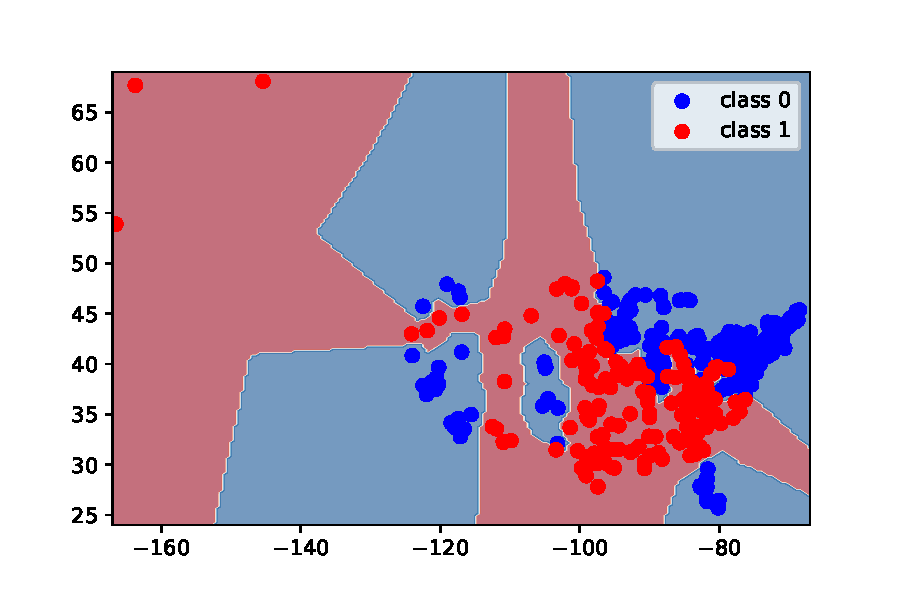
\includegraphics[width=3in]{../figs/q3_3_myKNN(k=1)}
\end{figure}
\gre{
\begin{itemize}
	\item The following figure is for KNighborsClassifier from scikit-learn.
\end{itemize}}
\begin{figure}[H]
	\centering
	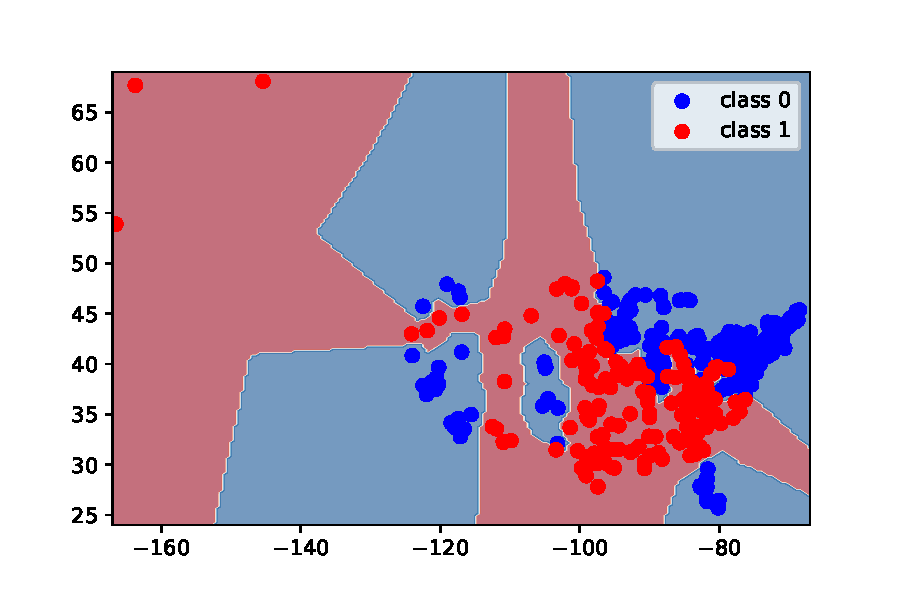
\includegraphics[width=3in]{../figs/q3_3_KNeighbors(k=1)}
\end{figure}
\item Why is the training error $0$ for $k=1$? \\
\gre{Answer:
\begin{itemize}
	\item Because we are choosing the label itself as predicted value when we set k=1 for KNN, which means we are simply copy the label itself.
\end{itemize}}
\item If you didn't have an explicit test set, how would you choose $k$? \\
\gre{Answer:
	\begin{itemize}
		\item We can use cross validation.
\end{itemize}}}}


\section{Random Forests}

\subsection{Implementation}
\rubric{code:4,reasoning:3}

The file \emph{vowels.pkl} contains a supervised learning dataset where we are trying to predict which of the 11 ``steady-state'' English vowels that a speaker is trying to pronounce.

You are provided with a \texttt{RandomStump} class that differs from
\texttt{DecisionStumpInfoGain} in that
it only considers $\lfloor \sqrt{d} \rfloor$ randomly-chosen features.\footnote{The notation $\lfloor x\rfloor$ means the ``floor'' of $x$, or ``$x$ rounded down''. You can compute this with \texttt{np.floor(x)} or \texttt{math.floor(x)}.}
You are also provided with a \texttt{RandomTree} class that is exactly the same as
\texttt{DecisionTree} except that it uses \texttt{RandomStump} instead of
\texttt{DecisionStump} and it takes a bootstrap sample of the data before fitting.
In other words, \texttt{RandomTree} is the entity we discussed in class, which
makes up a random forest.

If you run \texttt{python main.py -q 4} it will fit a deep \texttt{DecisionTree}
using the information gain splitting criterion. You will notice that the model overfits badly.




\blu{
\enum{
\item Why doesn't the random tree model have a training error of 0?\\
\gre{Answer:
	\begin{itemize}
		\item Because random tree model uses bootstrapping. For every bootstrap example, it only uses a subset of the whole dataset. so, even if it can get zero training error for every subset of data, it can not guarantee 0 training error overall for the whole dataset.
	\end{itemize}
}
\item Create a class \texttt{RandomForest} in a file called \texttt{random\string_forest.py} that takes in hyperparameters \texttt{num\string_trees} and \texttt{max\string_depth} and
fits \texttt{num\string_trees} random trees each with maximum depth \texttt{max\string_depth}. For prediction, have all trees predict and then take the mode. \\
\gre{Answer:
	\begin{itemize}
		\item Refer to code $"random_forest.py" $ for details.
	\end{itemize}}
\item Using 50 trees, and a max depth of $\infty$, report the training and testing error. Compare this to what we got with a single \texttt{DecisionTree} and with a single \texttt{RandomTree}. Are the results what you expected? Discuss. \\
\gre{Answer:
	\begin{itemize}
		\item The training error is 0 and the testing error is 0.174. The testing error is better than $DecisionTree$ and a single $RandomTree$. It's what we would expect.
\end{itemize}}
\item Compare your implementation with scikit-learn's \texttt{RandomForestClassifier} for both speed and accuracy, and briefly discuss. You can use all default hyperparameters if you wish, or you can try changing them. \\
\gre{Answer:
	\begin{itemize}
		\item The accuracies for RandomForestClassifier and RandomForest are pretty similar. Besides, sklearn's implementation is much faster.
\end{itemize}}
}
}

\section{Clustering}

If you run \verb|python main.py -q 5|, it will load a dataset with two features
and a very obvious clustering structure. It will then apply the $k$-means algorithm
with a random initialization. The result of applying the
algorithm will thus depend on the randomization, but a typical run might look like this:
\centerfig{.5}{../figs/kmeans_basic.png}
(Note that the colours are arbitrary -- this is the label switching issue.)
But the `correct' clustering (that was used to make the data) is this:
\centerfig{.5}{../figs/kmeans_good.png}


\subsection{Selecting among $k$-means Initializations}
\rubric{reasoning:5}

If you run the demo several times, it will find different clusterings. To select among clusterings for a \emph{fixed} value of $k$, one strategy is to minimize the sum of squared distances between examples $x_i$ and their means $w_{y_i}$,
\[
f(w_1,w_2,\dots,w_k,y_1,y_2,\dots,y_n) = \sum_{i=1}^n \norm{x_i - w_{y_i}}_2^2 = \sum_{i=1}^n \sum_{j=1}^d (x_{ij} - w_{y_ij})^2.
\]
 where $y_i$ is the index of the closest mean to $x_i$. This is a natural criterion because the steps of $k$-means alternately optimize this objective function in terms of the $w_c$ and the $y_i$ values.

 \blu{\enum{
 \item In the \texttt{kmeans.py} file, add a new function called \texttt{error} that takes the same input as the \texttt{predict} function but that returns the value of this above objective function.
 \item What trend do you observe if you print the value of this error after each iteration of the $k$-means algorithm?
 \item Using the \texttt{plot\_2dclustering} function defined in \texttt{main.py}, output the clustering obtained by running $k$-means 50 times (with $k=4$) and taking the one with the lowest error. Submit your plot.
 \item Looking at the hyperparameters of scikit-learn's \texttt{KMeans}, explain the first four (\texttt{n\_clusters}, \texttt{init}, \texttt{n\_init}, \texttt{max\_iter}) very briefly.
 }}


 \gre{ Answer:
 \begin{enumerate}
     \item Refer to the code in file kmeans.py
     \item The error will decrease monotonically with the iteration
     \item refer to the code in the file main.py to see how we choose the clustering with the lowest error, the clustering is showed in the following figure.
     \item n\_cluster: the number of clusters to form, which refer to number "k" for means; init:initialization method by applying k-means++; n\_init: the number of k-means algorithm to be run with different initialization; max\_iter: maximum iteration for each fun of k-means algorithm
 \end{enumerate}
 }
  \centerfig{.5}{../figs/kmeans_lowest_error.png}


 \subsection{Selecting $k$ in $k$-means}
\rubric{reasoning:5}

 We now turn to the task of choosing the number of clusters $k$.

 \blu{\enum{
 \item Explain why we should not choose $k$ by taking the value that minimizes the \texttt{error} function.
 \item Explain why even evaluating the \texttt{error} function on test data still wouldn't be a suitable approach to choosing $k$.
 \item Hand in a plot of the minimum error found across 50 random initializations, as a function of $k$, taking $k$ from $1$ to $10$.
 \item The \emph{elbow method} for choosing $k$ consists of looking at the above plot and visually trying to choose the $k$ that makes the sharpest ``elbow" (the biggest change in slope). What values of $k$ might be reasonable according to this method? Note: there is not a single correct answer here; it is somewhat open to interpretation and there is a range of reasonable answers.
 }}
\gre{Answer:
\begin{enumerate}
    \item The larger the $k$ is, the smaller the distance based error will be. Therefore, if we choose $k$ by minimizing the error, we will finally get that $k$ is equal to the number of examples of input $X$. This will lead to overfitting, and we can not learn too much from the clustering results, and it is hard to assign the new example to any cluster.
    \item The choice of $K$ is more related to the distribution of data.
    Taking the the clustering example mentioned in the class as a case. In that example, there are four obvious clusters in the data set, and $k=4$ is enough to differentiate examples in different cluster. However, if we evaluate the error, there is still a chance that we may want to increase $k$, and separate each cluster into even smaller sub-clusters. These sub-clusters can not reflect the real grouping properties of the examples in the data set.
    \item The plotted figure is shown as follows.
    \item We may choose $k=3$ or $4$.
\end{enumerate}
}
  \centerfig{.5}{../figs/error_with_k.png}

\subsection{Density-Based Clustering}
\rubric{reasoning:2}

If you run \texttt{python main.py -q 5.3},
it will apply the basic density-based clustering algorithm to the dataset from the previous part, but with some outliers added.
The final output should look somewhat like this:\\
\fig{.49}{../figs/density}\fig{.49}{../figs/density2}\\
(The right plot is zoomed in to show the non-outlier part of the data.)
Even though we know that each object was generated from one of four clusters (and we have 4 outliers),
 the algorithm finds 6 clusters and does not assign some of the original non-outlier
  objects to any cluster. However, the clusters will change if we change the parameters
  of the algorithm. Find and report values for the two
  parameters, \texttt{eps} (which we called the ``radius'' in class) and \texttt{minPts},
   such that the density-based clustering method finds:
\blu{\enum{
\item The 4 ``true" clusters.
\item 3 clusters (merging the top two, which also seems like a reasonable interpretaition).
\item 2 clusters.
\item 1 cluster (consisting of the non-outlier points).
}
}
\gre{ Answer:
Referring to the document of sklear.cluster.DBSCAN, and the introduction in Wikipedia, we learned that in density based clustering, clusters are defined as areas of higher density than the remainder of the data set.
For DBSCAN method, core samples of high density are first found and clusters are expanded from them.
For the two parameters eps and minPts, eps represents the maximum distance between two samples for them to be considered as in the same neighborhood.
minPts, which is min\_samples in the code, represents the number of samples in a neighborhood for a point to be considered as a core point.
In the following answers, we fix minPts as 3, and adjust eps, considering that eps will affect more on the number of clusters.
\begin{enumerate}
    \item can not find
    \item eps = 9
    \item eps = 14
    \item eps = 20
\end{enumerate}
}



\section{Very-Short Answer Questions}
\rubric{reasoning:13}

\blu{Write a short one or two sentence answer to each of the questions below}. Make sure your answer is clear and concise.

\enum{
\item What is an advantage of using a boxplot to visualize data rather than just computing its mean and variance?
\item What is a reason that the the data may not be IID in the email spam filtering example from lecture?
\item What is the difference between a validation set and a test set?
\item Why can't we (typically) use the training error to select a hyper-parameter?
\item What is the effect of $n$ on the optimization bias (assuming we use a parametric model).
\item What is an advantage and a disadvantage of using a large $k$ value in $k$-fold cross-validation.
\item Why can we ignore $p(x_i)$ when we use naive Bayes?
\item For each of the three values below in a naive Bayes model, say whether it's a parameter or a hyper-parameter:
\begin{enumerate}
\item Our estimate of $p(y_i)$ for some $y_i$.
\item Our estimate of $p(x_{ij} \cond y_i)$ for some $x_{ij}$ and $y_i$.
\item The value $\beta$ in Laplace smoothing.
\end{enumerate}
\item What is the effect of $k$ in KNN on the two parts (training error and approximation error) of the fundamental trade-off. Hint: think about the extreme values.
\item Suppose we want to classify whether segments of raw audio represent words or not. What is an easy way to make our classifier invariant to small translations of the raw audio?
\item Both supervised learning and clustering models take in an input $x_i$ and produce a label $y_i$. What is the key difference?
\item Suppose you chose $k$ in $k$-means clustering (using the squared distances to examples) from a validation set instead of a training set. Would this work better than using the training set (which just chooses the largest value of $k$)?
\item In $k$-means clustering the clusters are guaranteed to be convex regions. Are the areas that are given the same label by KNN also convex?
}
\gre{Answer:
\begin{enumerate}
    \item Mean and variance sometimes can not fully represent the properties of data, as different sets of data may have totally different distributions. However, boxplot includes minimum, first quartile, median, third quartile, and maximum, and can well display the distribution of data.
    \item Some key words for spam email characterization are closely related with each other.
    \item According to golden rule, we can not look at the test data during the training phase, thus can not estimate the test error during training. Validation set is divided from the trainning set and can be used to approximate test error with validation error.
    Validation set is used for model selection and test set is for final model to calculate the test error.
    \item To avoid overfitting.
    \item The larger $n$ is, the smaller the optimization bias will be.
    \item Advantage: Can help solve the problem of overfitting and get more accurate results.
    Disadvantage: May have high computation cost.
    \item In naive Bayes, what we want to do is to compare different conditional probabilities and choose the one with highest conditional probability. Since different conditional probabilities all share the probability $p(x_i)$, it will not affect the comparison.
    \item (a) parameter; (b) parameter; (c) hyper-parameter
    \item When $k$ is very small, the training error is small but the approximation error is large. When $k$ increases, the training error is large but the approximation error is small.
    \item Add the translations of the raw audio to the training set.
    \item For supervised learning, there is a training set to indicate the correct output $y$ based on the input $x$. For clustering model, there is no correct output $y$.
    \item It will work better.
    \item No. For k-means clustering, the areas are formed by perpendicular bisectors between any two of the mean points.
    For KNN, for example, when $k=1$, the areas are formed  by perpendicular bisectors between any two examples, which can not guarantee the convexity of the area. Actually, even for k-means clustering, when $k=N$, the convexity also can not be guaranteed.
\end{enumerate}
}


\end{document}
